\documentclass[12pt, titlepage]{article}

\usepackage{booktabs}
\usepackage{tabularx}
\usepackage{hyperref}
\hypersetup{
    colorlinks,
    citecolor=black,
    filecolor=black,
    linkcolor=red,
    urlcolor=blue
}
\usepackage[round]{natbib}
\usepackage[none]{hyphenat}
\usepackage{amssymb}
\usepackage{enumitem}
\usepackage[many]{tcolorbox}
\usepackage{mdframed}
\usepackage{parskip}
\usepackage{longtable}
\usepackage{diagbox}
\usepackage{float}
\usepackage{listings}

%% Comments

\usepackage{color}

\newif\ifcomments\commentstrue %displays comments
%\newif\ifcomments\commentsfalse %so that comments do not display

\ifcomments
\newcommand{\authornote}[3]{\textcolor{#1}{[#3 ---#2]}}
\newcommand{\todo}[1]{\textcolor{red}{[TODO: #1]}}
\else
\newcommand{\authornote}[3]{}
\newcommand{\todo}[1]{}
\fi

\newcommand{\wss}[1]{\authornote{blue}{SS}{#1}} 
\newcommand{\plt}[1]{\authornote{magenta}{TPLT}{#1}} %For explanation of the template
\newcommand{\an}[1]{\authornote{cyan}{Author}{#1}}

%% Common Parts

\newcommand{\progname}{ProgName} % PUT YOUR PROGRAM NAME HERE
\newcommand{\authname}{Team \#, Team Name
\\ Student 1 name
\\ Student 2 name
\\ Student 3 name
\\ Student 4 name} % AUTHOR NAMES                  

\usepackage{hyperref}
    \hypersetup{colorlinks=true, linkcolor=blue, citecolor=blue, filecolor=blue,
                urlcolor=blue, unicode=false}
    \urlstyle{same}
                                


\begin{document}

\title{Verification and Validation Report: \progname} 
\author{\authname}
\date{\today}
  
\maketitle

\pagenumbering{roman}

\section{Revision History}

\begin{tabularx}{\textwidth}{p{3cm}p{2cm}X}
\toprule {\bf Date} & {\bf Version} & {\bf Notes}\\
\midrule
03/01/2024 & 0.0 & Initial Document \\
03/02/2024 & 0.1 & Completed Symbols, Abbreviations and Acronyms, Automated Testing \\
03/04/2024 & 0.2 & Worked on Functional Requirements Evaluation, Nonfunctional Requirements Evaluation \\
03/05/2024 & 0.3 & Worked on Functional Requirements Evaluation, Nonfunctional Requirements Evaluation, Completed Changes due to Testing \\
03/06/2024 & 0.4 & Completed Functional Requirements Evaluation, Nonfunctional Requirements Evaluation, Unit Testing, Trace to Requirements, Reflection \\
03/06/2024 & 0.5 & Completed Trace to Modules, Code Coverage Metrics; formatting and final review \\
\bottomrule
\end{tabularx}

~\newpage

\section{Symbols, Abbreviations and Acronyms}
The following table, Table \ref{tab:symbsAbbrevsAcros}, includes the definitions and descriptions of all relevant symbols, abbreviations and acronyms used throughout this VnV Report document.

\renewcommand{\arraystretch}{1.2}
\begin{table}[H]
    \centering
    \label{tab:symbsAbbrevsAcros}
    \begin{tabular}{p{1.25in}p{3.75in}}
        \toprule
        \textbf{Symbol, Abbreviation or Acronym} & \textbf{Definition or Description} \\
        \midrule
        AI/ML & Artificial Intelligence/Machine Learning \\
        AUC & Area Under (ROC) Curve \\
        BUC & Business Use Case \\
        DICOM & Digital Imaging and Communications in Medicine, the standard for medical images to ensure data and quality necessary for clinical use.\\
        FR & Functional Requirement \\
        ICU & Intensive Care Unit \\
        IT & Information Technology \\
        MC & Mandated Constraints \\
        MG & Module Guide \\
        MIS & Module Interface Specification \\
        NFR & Non-functional Requirement \\
        PoC & Proof of Concept\\
        ROC curve & Receiver Operating Characteristic curve, a graph to show the performance of a model, plots true positive rate and false positive rate \\
        SRS & Software Requirements Specification \\
        T & Test \\
        TC & Test Case \\
        VnV & Verification and Validation \\
        \bottomrule
    \end{tabular}\\
    \caption{Symbols, Abbreviations and Acronyms}
\end{table}

\newpage

\tableofcontents

\listoftables %if appropriate

\listoffigures %if appropriate

\newpage

\pagenumbering{arabic}

This document intends to describe in detail the testing performed and the subsequent results in the verification and validation process of (NAME). In detail, the document outlines the evaluation of Functional system tests, Non Functional tests, and Unit tests. The Functional and Non Functional tests and their connection to the requirements can be found in the VnV Plan. As well, the unit tests are based on the individual modules that can be found in the MIS.  

\section{Functional Requirements Evaluation}
The following are the test cases carried out as part of the functional requirements evaluation of the project software application. For each test case, the test case name, input, expected output, actual output, whether the actual output matched the expected output, and the relevant FR(s) are outlined in detail in this section. The test cases are organized into subsections based on what overarching functionality is being tested (i.e. handling input data, display, classification of diseases, access of database and authorization).

\subsection{Handling Input Data}
In this subsection, the test cases evaluating the software application for its input data handling functionalities are outlined in detail alongside the testing results. \\

\begin{mdframed}[linewidth=0.5mm]
  \textbf{Test Case Name:} DICOM Input Acceptance (TC.1) \par
  \textbf{Input:} A sample chest X-ray image in DICOM format. \par
  \textbf{Expected Output:} The DICOM input is accepted and converted into a JPEG successfully, with no error messages or system anomalies. \par
  \textbf{Actual Output:} The given DICOM image is converted to JPEG format. \par
  \textbf{Expected and Actual Output Match:} True \par
  \textbf{Relevant Functional Requirement(s):} FR.1, FR.7
\end{mdframed}

\begin{mdframed}[linewidth=0.5mm]
  \textbf{Test Case Name:} Non-DICOM Input Rejection (TC.2) \par
  \textbf{Input:} A sample chest X-ray image in a format other than DICOM. \par
  \textbf{Expected Output:} The non-DICOM input is rejected, and an appropriate error message is returned. \par
  \textbf{Actual Output:} The image is rejected and an error message is returned. \par
  \textbf{Expected and Actual Output Match:} True \par
  \textbf{Relevant Functional Requirement(s):} FR.1
\end{mdframed}

\begin{mdframed}[linewidth=0.5mm]
  \textbf{Test Case Name:} DICOM conversion to JPEG (TC.3) \par
  \textbf{Input:} A sample chest X-ray image DICOM format. \par
  \textbf{Expected Output:} The output is the same X-ray image in JPEG format. \par
  \textbf{Actual Output:} The given image in DICOM format is displayed as a JPEG image. \par
  \textbf{Expected and Actual Output Match:} True \par
  \textbf{Relevant Functional Requirement(s):} FR.8
\end{mdframed}

\subsection{Display}
In this subsection, the test cases evaluating the software application for its display functionalities are outlined in detail alongside the testing results. \\

\begin{mdframed}[linewidth=0.5mm]
  \textbf{Test Case Name:} Image Display Correctness (TC.4) \par
  \textbf{Input:} Processed chest X-ray images with known medical conditions. \par
  \textbf{Expected Output:} The correct display of chest X-ray images on the user interface, and reflects the processed medical conditions accurately. \par
  \textbf{Actual Output:} The given chest X-ray image and the identified medical condition is correctly displayed. \par
  \textbf{Expected and Actual Output Match:} True \par
  \textbf{Relevant Functional Requirement(s):} FR.2, FR.3
\end{mdframed}

\begin{mdframed}[linewidth=0.5mm]
  \textbf{Test Case Name:} Report and Terms Correctness (TC.5) \par
  \textbf{Input:} Processed chest X-ray images with known medical conditions. \par
  \textbf{Expected Output:} The correct display of medical reports and associated terms on the user interface accurately reflects the processed information. \par
  \textbf{Actual Output:} The correct diagnosis report for the processed image is displayed. \par
  \textbf{Expected and Actual Output Match:} True \par
  \textbf{Relevant Functional Requirement(s):} FR.4, FR.5
\end{mdframed}

\subsection{Classification of Diseases}
\hypertarget{disClasCorPerf}
In this subsection, the test cases evaluating the software application for its classification of disease functionalities are outlined in detail alongside the testing results. \\

\begin{mdframed}[linewidth=0.5mm]
  \textbf{Test Case Name:} Disease Classification Correctness Performance (TC.6) \par
  \textbf{Input:} DICOM chest X-ray images, approximately 20\% of the dataset DATASET\_NAME will be reserved and used to run this test/experiment, with known medical conditions representing various diseases. \par
  \textbf{Expected Output:} The AUC for the ROC curves for the classification of diseases based on the expected area under the ROC curves is given in Table 6 in the SRS. \par
  \textbf{Actual Output:} The expected AUC of each disease classification matches the expected AUC given in Table 6 of the SRS. \par
  \textbf{Expected and Actual Output Match:} True \par
  \textbf{Relevant Functional Requirement(s):} FR.6
\end{mdframed}

\subsection{Access of Database}
In this subsection, the test cases evaluating the software application for its access to database functionalities are outlined in detail alongside the testing results. \\

\begin{mdframed}[linewidth=0.5mm]
  \textbf{Test Case Name:} Database Search Functionality (TC.7) \par
  \textbf{Input:} User-initiated search queries for patient records based on specified criteria such as patient ID (unique), name, date of X-ray, or medical condition(s). \par
  \textbf{Expected Output:} The accurate retrieval of patient records matching the specified search criteria, is displayed on the user interface. \par
  \textbf{Actual Output:} The requested patient data is accurately displayed to the user. \par
  \textbf{Expected and Actual Output Match:} True \par
  \textbf{Relevant Functional Requirement(s):} FR.6, FR.9, FR.11
\end{mdframed}

\subsection{Authorization}
\hypertarget{Auth}
In this subsection, the test cases evaluating the software application for its authorization functionalities are outlined in detail alongside the testing results. \\

\begin{mdframed}[linewidth=0.5mm]
  \textbf{Test Case Name:} Correct User Login (TC.8) \par
  \textbf{Input:} User-initiated login attempts with valid credentials. \par
  \textbf{Expected Output:} The successful login of authorized users, granting them access to the system. \par
  \textbf{Actual Output:} The authorized user is able to log in with valid credentials and be granted access to the system. \par
  \textbf{Expected and Actual Output Match:} True \par
  \textbf{Relevant Functional Requirement(s):} FR.10
\end{mdframed}

\begin{mdframed}[linewidth=0.5mm]
  \textbf{Test Case Name:} Incorrect User Login (TC.9) \par
  \textbf{Input:} User-initiated login attempts with invalid credentials. \par
  \textbf{Expected Output:} The rejection of login attempts with invalid credentials, accompanied by the appropriate error message. \par
  \textbf{Actual Output:} The user login attempts with invalid credentials are rejected, and the user is not granted access to the system. \par
  \textbf{Expected and Actual Output Match:} True \par
  \textbf{Relevant Functional Requirement(s):} FR.10
\end{mdframed}

\begin{mdframed}[linewidth=0.5mm]
  \textbf{Test Case Name:} Creation of New Authorized User (TC.10) \par
  \textbf{Input:} User-initiated creation of a new authorized user account through the user interface. \par
  \textbf{Expected Output:} The expected result is the successful creation of a new authorized user account recorded and saved in the system. \par
  \textbf{Actual Output:} The new authorized user account is created successfully and saved in the system. \par
  \textbf{Expected and Actual Output Match:} True \par
  \textbf{Relevant Functional Requirement(s):} FR.10
\end{mdframed}

\section{Nonfunctional Requirements Evaluation}
The following are the test cases carried out as part of the nonfunctional requirements evaluation of the project software application. For each test case, the test case name, input, expected output, actual output, whether the actual output matched the expected output, and the relevant NFR(s) are outlined in detail in this section. The test cases are organized into subsections based on what overarching property is being tested (i.e. usability, performance and security).

\subsection{Usability}
In this subsection, the test cases evaluating the software application for its usability properties are outlined in detail alongside the testing results. \\

\begin{mdframed}[linewidth=0.5mm]
  \textbf{Test Case Name:} Software Application Usability I (TC.16A) \par
  \textbf{Input:} Usability testers will attempt to perform a given set of tasks (e.g. retrieving patient data) using the software application's GUI. \par
  \textbf{Expected Output:} The usability testers will perform the tasks and complete a survey documenting their experiences and thoughts on the GUI's usability. \par
  \textbf{Actual Output:} The testers submitted a survey on their experience using the GUI. \par
  \textbf{Expected and Actual Output Match:} True \par
  \textbf{Relevant Nonfunctional Requirement(s):} NF.A0, NF.C0, NF.EUR0, NF.LR0, NF.UPR0
\end{mdframed}

\begin{mdframed}[linewidth=0.5mm]
  \textbf{Test Case Name:} Software Application Usability II (TC.16B) \par
  \textbf{Input:} A given set of tasks (e.g. retrieving patient data) using the software application's GUI will be completed during a walk-through and demo with the supervisor and/or other peers. \par
  \textbf{Expected Output:} The supervisor and/or peers will give feedback documenting their thoughts on the GUI's usability. \par
  \textbf{Actual Output:} The supervisor was given a walkthrough and demo of the software application and gave verbal feedback to the team that was documented. See the Changes due to Testing section for more information on the exact feedback. \par
  \textbf{Expected and Actual Output Match:} True \par
  \textbf{Relevant Nonfunctional Requirement(s):} NF.A0, NF.C0, NF.EUR0, NF.LR0 and NF.UPR0
\end{mdframed}
    
\subsection{Performance}
In this subsection, the test cases evaluating the software application for its performance properties are outlined in detail alongside the testing results. \\

%(FAST VS RESPONSE TIME?)
%(ADD FOR ML MODEL. ON A LARGE DATASET. METRIC - AREA UNDER ROC CURVE)
\begin{mdframed}[linewidth=0.5mm]
  \textbf{Test Case Name:} System Response Time (TC.12) \par
  \textbf{Input:} Automated requests for all the various system functionalities, including image processing and database searches. Additionally, this includes website launch and load time. \par
  \textbf{Expected Output:} The system provides responses within the defined acceptable time thresholds for each functionality as specified in section 3.3.1 of the SRS. \par
  \textbf{Actual Output:} The system responses are provided within the defined acceptable time thresholds for each functionality as specified.
  
  The average load time of the website from launch was 4 seconds. 
  \par
  \textbf{Expected and Actual Output Match:} True \par
  \textbf{Relevant Nonfunctional Requirement(s):} NF.SLR0

  \begin{table}[H]
  \centering
    \label{tab:websiteLoadTime}
    \begin{tabular}{|c|c|}
    \hline
       Runs  & Time (seconds) \\
       \hline
        \#1 & 3.2  \\
        \#2 & 3.8  \\
        \#3 & 3.8  \\
        \#4 & 4.2  \\
        \#5 & 4.4  \\
        \#6 & 5.6 \\
        \hline
    \end{tabular}
    \caption{Website Load Time}
  \end{table}

  \begin{figure}[H]
      \centering
      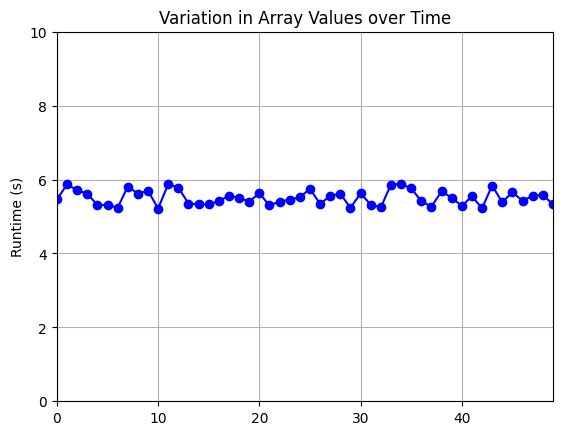
\includegraphics[width=0.75\linewidth]{output1.png}
      \caption{Variation in ML Model Runtime}
      \label{fig:enter-label}
  \end{figure}
  \begin{figure}[H]
      \centering
      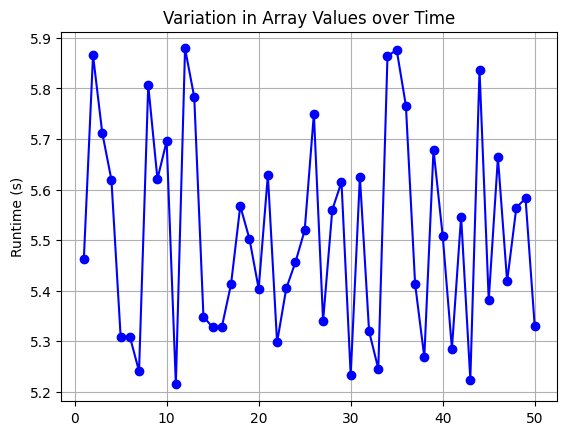
\includegraphics[width=0.75\linewidth]{output2.png}
      \caption{Variation in ML Model Runtime (Expanded Y-Axis)}
      \label{fig:enter-label}
  \end{figure}
\end{mdframed}

\begin{mdframed}[linewidth=0.5mm]
  \textbf{Test Case Name:} Accuracy of the ML Model (TC.13) \par
  \textbf{Input:} See FR test case \hyperlink{disClasCorPerf}{Disease Classification Correctness Performance} for reference \par
  \textbf{Expected Output:} Likewise refer to \hyperlink{disClasCorPerf}{Disease Classification Correctness Performance} for more details. \par
  \textbf{Actual Output:} AUC of each disease is accurate according to Table 6 in the SRS. \par
  \textbf{Expected and Actual Output Match:} True \par
  \textbf{Relevant Nonfunctional Requirement(s):} NF.PAR0
\end{mdframed}

\begin{mdframed}[linewidth=0.5mm]
  \textbf{Test Case Name:} Patient Data Collection (TC.14) \par
  \textbf{Input:} A New patient is added to the system. \par
  \textbf{Expected Output:} The system will retain the patient name, past diagnoses, assigned physician, past visit dates and other relevant data, while not retaining any unnecessary data. \par
  \textbf{Actual Output:} The system only retains the needed patient data to identify patients and link them to their chest X-ray images and scan results, medical history, assigned physician and other relevant data. \par
  \textbf{Expected and Actual Output Match:} True \par
  \textbf{Relevant Nonfunctional Requirement(s):} NF.SCR0
\end{mdframed}

\begin{mdframed}[linewidth=0.5mm]
  \textbf{Test Case Name:} Capacity (TC.15) \par
  \textbf{Input:} Three sample chest X-ray images in DICOM format divided between three computers using the system. \par
  \textbf{Expected Output:} The correct display of chest X-ray images on the user interface, reflects all the processed medical conditions accurately for each upload. \par
  \textbf{Actual Output:} The images are correctly displayed on the user interface with all the processed information. \par
  \textbf{Expected and Actual Output Match:} True \par
  \textbf{Relevant Nonfunctional Requirement(s):} NF.CR0
\end{mdframed}

\subsection{Security}
In this subsection, the test cases evaluating the software application for its security properties are outlined in detail alongside the testing results. \\

\begin{mdframed}[linewidth=0.5mm]
  \textbf{Test Case Name:} Data Encryption/Secure Access (TC.11) \par
  \textbf{Input:} Software Application requests patient data as an authenticated user. \par
  \textbf{Expected Output:} The encrypted data (not plain text data) is returned only for an authenticated user. \par
  \textbf{Actual Output:} The data is returned only for an authenticated user (non-authenticated are denied access to the patient data). \par
  \textbf{Expected and Actual Output Match:} True \par
  \textbf{Relevant Nonfunctional Requirement(s):} NF.IR0, NF.PR1
\end{mdframed}

Also, see \hyperlink{Auth}{Authorization} in the Functional Requirements Evaluation section for NF.AR0, NF.AR1, NF.PR0 and NF.PR1 as they all relate to limiting access to records for authorized individuals.
  
% \section{Comparison to Existing Implementation} 

% This section will not be appropriate for every project.

\section{Unit Testing}

Unit testing was conducted on the different functions in each of the modules. The goal of these tests was to verify the correctness of independent units of code based on the separation of concerns in the system. The table below lists the functions tested in the corresponding modules, and the results of those tests.

\begin{table}[H]
  \centering
  \label{tab:unitTestingResults}
  \begin{tabular}{|c|c|c|}
    \hline
    \textbf{Module} & \textbf{Function Tested} & \textbf{Result} \\
    \hline
    ChestXRayRead & dcmFileValid & Passed \\
             & parseDcm & Passed \\
             & convertDcm2Jpg & Passed \\
    \hline
    ResultGen & reportResults & Passed \\      
    \hline
    RepCompGen & nlpGen & Passed \\
                & processImage & Passed \\
    \hline
    AIModel & processImage & Passed \\
            & predictions & Passed \\ 
    \hline
    Backend & createANewUser & Passed \\
            & loginAUser & Passed \\
            & logoutAUser & Passed \\
            & deleteAUser & Passed \\
    \hline
    DatabaseOps & writeUserData & Passed \\
                & readUserData & Passed \\
                & createNewUserData & Passed \\
                & deleteUserData & Passed \\
    \hline
    UserAuthMgmt & createNewUser & Passed \\
                 & loginUser & Passed \\
                 & logoutUser & Passed \\
                 & deleteUser & Passed \\
    \hline
    AppGUI & displayLoginPage & passed \\
            & displayScanPage & passed \\
            & displayResultsPage & passed \\
    \hline
    PerformScan & initiateScan & passed\\
    \hline
    ViewResults & displayReport & passed \\
    \hline
    
  \end{tabular}
  \caption{Unit Testing Results}
\end{table}

Overall, unit testing serves as a fundamental component of our software development process, enabling us to maintain code quality, identify and fix defects early, and ensure the overall reliability and robustness of our software application. We aim to achieve thorough test coverage across the entire software stack, from frontend user interfaces to backend business logic and data processing pipelines. By adhering to best practices in unit testing and continuously refining our test suites, we can deliver a high-quality software product that meets the functional requirements, performance expectations, and user satisfaction criteria outlined in our project specifications.

\section{Changes Due to Testing}

% \wss{This section should highlight how feedback from the users and from 
% the supervisor (when one exists) shaped the final product.  In particular 
% the feedback from the Rev 0 demo to the supervisor (or to potential users) 
% should be highlighted.}
During the testing phase, several important changes were identified and implemented based on feedback from users and supervisors, particularly following the Rev 0 demo. These changes were aimed at enhancing the functionality, usability, and overall effectiveness of the software application. Here are the key changes:
\begin{itemize}
    \item \textbf{Integration of NLP Report Generation:}  Initially, generating NLP reports from chest X-ray images was a stretch goal. However, based on feedback and the importance of this functionality, it was elevated to one of the project's main goals. \\
    A new feature was introduced to generate NLP reports from chest X-ray images. This involved developing a separate ML model dedicated to producing textual reports, distinct from the model used for disease identification. By including this capability, the application can provide comprehensive diagnostic insights in textual format, enhancing its utility for healthcare professionals.
    \item \textbf{Modification of Image Upload Process:} Based on feedback and usability considerations, the process for uploading images or DICOM files was restructured. Instead of uploading images/DICOM files directly, it was decided to assume that the files had already been uploaded to the server. As a result, the user interface was modified to automatically populate relevant patient data and linked images/DICOM files when selecting a patient. This modification aimed to simplify the user experience and improve efficiency by eliminating redundant steps.
    \item \textbf{Store Results in Database:} To ensure comprehensive record-keeping and facilitate future reference, consideration was given to storing diagnostic results in the database. While this change was optional, it aimed to provide a centralized repository for patient data and corresponding analyses, enhancing data management capabilities and enabling further analysis and reporting.
    \item \textbf{Usability:} A majority of feedback received during our walk-through and revision 0 demo focused on the redundancy of information that needed to be uploaded to utilize the application. We've decided to update the UI to allow for the users to select from existing patients to conduct a study and allow new X-ray images the be the only new information required to conduct new studies. 
\end{itemize}

\section{Automated Testing}
\subsection{Linters}
The first step in our automated testing pipeline involves the use of linters such as Prettier, ESLint, Flake8, and Black. These tools are configured to run automatically upon code changes to enforce coding standards, detect syntax errors, and ensure consistent formatting across the entire codebase.
\begin{itemize}
    \item \textbf{Prettier:} Ensures consistent code formatting across the project, eliminating debates over style preferences and enhancing code readability.
    \item \textbf{ESLint:} Identifies problematic patterns or code that does not adhere to specified coding rules for TypeScript.
    \item \textbf{Flake8:} Performs linting for Python code, enforcing PEP 8 style guidelines and detecting syntax errors and code smells.
    \item \textbf{Black:} Enforces a consistent code style for Python, automatically formatting code to adhere to the Black code style. 
\end{itemize}

\subsection{Unit testing}
\begin{itemize}
    \item \textbf{Jest:} Jest is used to test the frontend components and functionalities of our application developed using React.js. We write Jest test cases to verify the behaviour of individual React components, including their rendering, state management, event handling, and integration with external libraries or APIs. By leveraging Jest's comprehensive testing capabilities, we ensure the robustness and correctness of our frontend codebase, allowing us to catch bugs and issues early in the development process.
    \item \textbf{Pytest:} Pytest is employed to test the backend logic, APIs, and data processing functionalities of our software application developed using Python. We create Pytest test suites to validate the functionality and performance of various backend modules, including data retrieval, processing, storage, and interaction with external services or databases. Pytest allows us to write concise and expressive test cases, enabling thorough testing of different aspects of our backend codebase. By leveraging Pytest's robust testing features, we ensure the correctness, stability, and efficiency of our backend implementation, facilitating the delivery of a high-quality software product.
\end{itemize}

% \subsection{Code coverage}
% To assess the effectiveness of our testing efforts, we utilize code coverage tools like Istanbul for JavaScript and Coverage.py for Python. These tools measure the percentage of code executed during testing, helping us identify areas of the codebase that may lack sufficient test coverage and require further attention.

\subsection{Continuous Integration}
Continuous Integration (CI) is seamlessly integrated into our development workflow using GitHub Actions, enabling automated testing to occur with every code change. CI workflows are configured to trigger automated tests on each pull request and push to the main branch, ensuring that any introduced changes undergo thorough testing before integration into the main codebase.
\begin{itemize}
    \item \textbf{Trigger:} CI workflows are triggered automatically on every pull request and push to the main branch, ensuring that all changes are validated before being merged.
    \item \textbf{Feedback:} Upon completion of the CI workflow, developers receive immediate feedback on the status of their code changes. If any tests fail, developers are alerted, allowing them to quickly address issues and iterate on their code.
\end{itemize}
    
\section{Trace to Requirements}
In this section, the traceability matrices linking the functional and non-functional requirements to the test cases are shown. \\

\begin{table}[H]
    \centering
    \label{tab:traceabilityMatrixforFunctionalRequirements}
    \hspace*{-1.25cm}
    \begin{tabular}{|c|c|c|c|c|c|c|c|c|c|c|}
        \hline
        \diagbox{FR}{TC} & TC.1 & TC.2 & TC.3 & TC.4 & TC.5 & TC.6 & TC.7 & TC.8 & TC.9 & TC.10 \\
        \hline
        FR1 & X & X & & & & & & & & \\
        \hline
        FR2 & & & & X & & & & & & \\
        \hline
        FR3 & & & & X & & & & & & \\
        \hline
        FR4 & & & & & X & & & & & \\
        \hline
        FR5 & & & & & X & & & & & \\
        \hline
        FR6 & & & & & & X & X & & & \\
        \hline
        FR7 & X & & & & & & & & & \\
        \hline
        FR8 & & & X & & & & & & & \\
        \hline
        FR9 & & & & & & & X & & & \\
        \hline
        FR10 & & & & & & & & X & X & X \\
        \hline
        FR11 & & & & & & & X & & & \\
        \hline
    \end{tabular}
    \caption{Traceability Matrix for Functional Requirements}
\end{table}

\begin{table}[H]
    \centering
    \label{tab:traceabilityMatrixforNonfunctionalRequirementsI}
    \hspace*{-1.25cm}
    \begin{tabular}{|c|c|c|c|c|c|c|c|c|c|c|}
        \hline
        \diagbox{NFR}{TC} & TC.1 & TC.2 & TC.3 & TC.4 & TC.5 & TC.6 & TC.7 & TC.8 & TC.9 & TC.10 \\
        \hline
        NF.PAR0 & & & & & & X & & & & \\
        \hline
        NF.RIAS0 & X & X & X & X & X & & & & & \\
        \hline
        NF.PR0 & X & X & X & X & X & & X & X & X & X \\
        \hline
        NF.SR0 & X & X & X & X & X & & X & X & X & X \\
        \hline
        NF.AR0 & & & & & & & & X & X & X \\
        \hline
        NF.AR1 & & & & & & & & X & X & X \\
        \hline
        NF.PR0 & & & & & & & & X & X & X \\
        \hline
        NF.PR1 & & & & & & & & X & X & X \\
        \hline
    \end{tabular}
    \caption{Traceability Matrix for Nonfunctional Requirements I}
\end{table}

\begin{table}[H]
    \centering
    \label{tab:traceabilityMatrixforNonfunctionalRequirementsII}
    \begin{tabular}{|c|c|c|c|c|c|c|}
        \hline
        \diagbox{NFR}{TC} & TC.11 & TC.12 & TC.13 & TC.14 & TC.15 & TC.16 \\
        \hline
        NF.A0 & & & & & & X \\
        \hline
        NF.EUR0 & & & & & & X \\
        \hline
        NF.LR0 & & & & & & X \\
        \hline
        NF.UPR0 & & & & & & X \\
        \hline
        NF.SLR0 & & X & & & & \\
        \hline
        NF.SCR0 & & & & X & & \\
        \hline
        NF.PAR0 & & & X & & & \\
        \hline
        NF.CR0 & & & & & X & \\
        \hline
        NF.PR0 & X & X & X & X & X & X \\
        \hline
        NF.SR0 & X & X & X & X & X & X \\
        \hline
        NF.IR0 & X & & & & & \\
        \hline
        NF.PR1 & X & & & & & \\
        \hline
        NF.C0 & & & & & & X \\
        \hline
    \end{tabular}
    \caption{Traceability Matrix for Nonfunctional Requirements II}
\end{table}

\section{Trace to Modules}
In this section, the traceability matrices linking the software modules to the test cases are shown. \\

\begin{table}[H]
    \centering
    \label{tab:traceabilityMatrixforModulesI}
    \hspace*{-1.25cm}
    \begin{tabular}{|c|c|c|c|c|c|c|c|c|c|c|}
        \hline
        \diagbox{NFR}{TC} & TC.1 & TC.2 & TC.3 & TC.4 & TC.5 & TC.6 & TC.7 & TC.8 & TC.9 & TC.10 \\
        \hline
        M1 & & & & & X & X & & & & \\
        \hline
        M2 & & & & & X & X & & & & \\
        \hline
        M3 & & & & & X & X & & & & \\
        \hline
        M4 & & & & & X & & & & & \\
        \hline
        M5 & & & & & X & & & & & \\
        \hline
        M6 & & & & & & & & X & X & X \\
        \hline
        M7 & & & & & & & & & & \\
        \hline
        M8 & & & & & & & & X & X & X \\
        \hline
        M9 & & & & & & & & & & \\
        \hline
        M10 & X & X & X & X & X & & X & X & X & X \\
        \hline
        M11 & X & X & X & X & X & & X & X & X & X \\
        \hline
        M12 & & & & & & & & X & X & X \\
        \hline
        M13 & X & X & X & X & X & & & & & \\
        \hline
        M14 & & & & X & X & & X & & & \\
        \hline
    \end{tabular}
    \caption{Traceability Matrix for Software Modules I}
\end{table}

\begin{table}[H]
    \centering
    \label{tab:traceabilityMatrixforModulesII}
    \begin{tabular}{|c|c|c|c|c|c|c|}
        \hline
        \diagbox{NFR}{TC} & TC.11 & TC.12 & TC.13 & TC.14 & TC.15 & TC.16 \\
        \hline
        M1 & & X & X & & X & X \\
        \hline
        M2 & & X & X & & X & X \\
        \hline
        M3 & & X & X & & X & X \\
        \hline
        M4 & & X & & & X & X \\
        \hline
        M5 & & X & & & X & X \\
        \hline
        M6 & X & X & & X & & X \\
        \hline
        M7 & X & X & & X & & X \\
        \hline
        M8 & X & X & & X & & X \\
        \hline
        M9 & & X & & X & & X \\
        \hline
        M10 & X & X & & X & X & X \\
        \hline
        M11 & X & X & & X & X & X \\
        \hline
        M12 & X & X & & X & & X \\
        \hline
        M13 & & X & & & X & X \\
        \hline
        M14 & & X & & & X & X \\
        \hline
    \end{tabular}
    \caption{Traceability Matrix for Software Modules II}
\end{table}

\section{Code Coverage Metrics}
In this section, the code coverage metrics are summarized for each software module. The code coverage values are given as percentages of code covered with a combination of automatic and/or unit tests. \\

\begin{table}[H]
    \centering
    \label{tab:CodeCovMetrics}
    \hspace*{-2cm}
    \begin{tabular}{|c|c|c|c|}
        \hline
        Module & Statement Coverage \% & Condition Coverage \% & Decision Coverage \% \\
        \hline
        M1: AIModel & 100 & 100 & 100 \\
        \hline
        M2: ChestXRayRead & 100 & 100 & 100 \\
        \hline
        M3: ResultGen & 100 & 100 & 100 \\
        \hline
        M4: NLPModel & 100 & 100 & 100 \\
        \hline
        M5: RepCompGen & 100 & 100 & 100 \\
        \hline
        M6: Backend & 100 & 100 & 100 \\
        \hline
        M7: DatabaseOps & 100 & 100 & 100 \\
        \hline
        M8: UserAuthMgmt & 100 & 100 & 100 \\
        \hline
        M9: MedInstInter & 100 & 100 & 100 \\
        \hline
        M10: AppController & 100 & 100 & 100 \\
        \hline
        M11: AppGUI & 100 & 100 & 100 \\
        \hline
        M12: Login & 100 & 100 & 100 \\
        \hline
        M13: PerfScan & 100 & 100 & 100 \\
        \hline
        M14: ViewResults & 100 & 100 & 100 \\
        \hline
    \end{tabular}
    \caption{Code Coverage Metrics}
\end{table}

% \bibliographystyle{plainnat}
% \bibliography{../../refs/References}

\newpage{}
\section*{Appendix --- Reflection}

% The information in this section will be used to evaluate the team members on the
% graduate attribute of Reflection.  Please answer the following question:

% \begin{enumerate}
%   \item In what ways was the Verification and Validation (VnV) Plan different
%   from the activities that were conducted for VnV?  If there were
%   differences, what changes required the modification in the plan?  Why did
%   these changes occur?  Would you be able to anticipate these changes in future
%   projects?  If there weren't any differences, how was your team able to 
%   predict a feasible amount of effort and the right tasks needed to build the
%   evidence that demonstrates the required quality?  (It is expected that most
% of teams will have had to deviate from their original VnV Plan.)
% \end{enumerate}

In reflecting on the Verification and Validation (VnV) Plan, it is evident that the actual activities deviated somewhat from the initial plan. Prior to development, our team outlined a VnV Plan based on our understanding of the project scope and requirements. Our VnV Plan provided a structured framework for verification and validation processes, outlining test case creation, execution, and analysis. However, as the development progressed, we realized that the scope of our actual implementation had evolved beyond what was initially envisioned.

For instance, we initially planned for the AI model to solely detect common chest diseases from X-ray images. However, during implementation, we decided to expand the functionality to include generating natural language processing (NLP) reports based on the detected conditions and incorporating new functionalities, such as enhanced data management capabilities, which were deemed essential for meeting user needs and project goals. Consequently, the VnV Plan had to be adapted to incorporate these new requirements and ensure comprehensive testing coverage. This underscored the importance of flexibility and adaptability in project management.

Reflecting on this experience, we acknowledge that our initial VnV Plan lacked a comprehensive understanding of the project's full scope and potential functionalities. We now recognize the importance of conducting thorough research and planning before finalizing the VnV Plan to anticipate potential changes in project scope more effectively. Additionally, better communication and collaboration among team members during the planning phase could have facilitated a clearer vision of the project's requirements and goals, helping to align the VnV Plan more closely with the actual implementation.

Looking ahead, incorporating more robust mechanisms for gathering requirements, conducting feasibility studies, anticipating potential scope changes and stakeholder feedback can help in designing a more flexible VnV Plan for future projects, enabling teams to accommodate adjustments without compromising the overall testing efficacy.

\end{document}
